\chapter{Podstawy teoretyczne}

Problem kategoryzacji obrazów wpisuje się w dziedzinę rozpoznawania obrazów. Zadanie to polega na rozpoznaniu przynależności różnych rodzajów obiektów do pewnych klas\cite{Tad91} i jest częścią większego zagadnienia, które określa się jako uczenie maszynowe.

\section{Uczenie maszynowe}

Uczenie maszynowe jest zagadnieniem interdyscyplinarnym z pogranicza informatyki, statystyki i sztucznej inteligencji, które zajmuje się tworzeniem systemów mogących doskonalić się za pomocą dostarczanych danych.

Systemy te ulegają nieustannej modyfikacji, zmieniają swoje wewnętrzne parametry po to by osiągnąć korzyści takie jak zwiększenie efektywności lub wydajności działania. Ważną cechą jest to, że jakkolwiek zmiany te zachodzą na podstawie czynników zewnętrznych to jednak dokonują się w systemie autonomicznie. System, który się uczy zmienia sam siebie na lepsze.\cite{CICHOSZ00}

\section{Uczenie nadzorowane i nienadzorowane}

W uczeniu maszynowym możemy wyróżnić dwa zasadnicze podejścia: uczenie nadzorowane (\emph{ang. supervised machine learning}) i nienadzorowane (\emph{ang. unsupervised machine learning}). Różnica pomiędzy nimi polega na obecności w uczeniu nadzorowanym tzw. nauczyciela, który stanowi źródło informacji trenującej. Posługując się analogiczną terminologią, system który podlega nauce określa się jako ucznia. Na rys. \ref{fig:supervised-learning} przedstawiono schemat uczenia maszynowego z użyciem nauczyciela.

\begin{figure}[h]
	\centering
	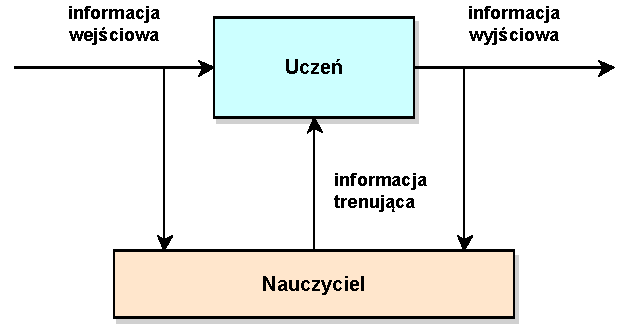
\includegraphics{graphics/01_podstawy_teoretyczne/supervised-learning.pdf}
	\caption{Uczenie maszynowe z nauczycielem \cite{CICHOSZ00}}
	\label{fig:supervised-learning}
\end{figure}

Uczeń otrzymuje od nauczyciela informację o tym jakiego komunikatu wyjściowego oczekuje w odpowiedzi na przykładowe informacje wejściowe. Mogą być one dostarczone np. w formie par składających się z wektorów danych oraz poprawnej odpowiedzi. Na podstawie przykładów, system ma wyuczyć się przyporządkowywania danych do odpowiednich odpowiedzi.

W zależności od typu odpowiedzi możemy wyróżnić dwa typowe rodzaje problemów, które stara się rozwiązać uczenie nadzorowane. Jeśli system ma przyporządkować do wektora wejściowego pojedynczą kategorię pochodzącą ze skończonego i dyskretnego zbioru kategorii, wówczas określamy ten problem jako problem kategoryzacji. Natomiast w przypadku przyporządkowywania odpowiedzi składającej się z jednej lub więcej zmiennych ciągłych, mówimy o problemie regresji.\cite{BISHOP06} Proces działania maszyny realizującej uczenie nadzorowane możemy podzielić na dwa etapy: etap treningu lub też nauki oraz etap polegający na rozwiązywania przynależności nowych wektorów wejściowych, który często określa się jako testowanie lub walidację.

W uczeniu nienadzorowanym nie występuje rola nauczyciela, a co za tym idzie, do systemu nie trafiają informacje treningowe. Wówczas dostępne są jedynie wektory wejściowe i na podstawie ich obserwacji uczeń ma nauczyć się odpowiednich odpowiedzi.\cite{CICHOSZ00} Podejście to zatem nie polega przyporządkowaniu wektorów do ustalonych wcześniej kategorii, lecz na znalezieniu pewnej ukrytej cechy pośród danych względem której można podzielić dane.\cite{VALPOLA} 

Rzeczywiste dane wejściowe mogą się różnić od przykładowych danych służących do wytrenowania systemu. Umiejętność udzielania poprawnej odpowiedzi na komunikaty, które różnią się od przykładowych danych określamy jako generalizacja.\cite{BISHOP06} 

Ze względu na specyfikę problemu, należałoby stwierdzić, że właściwym podejściem do zautomatyzowania procesu kategoryzacji zdjęć jest uczenie nadzorowane.

\section{Rozpoznawanie obrazów}
...

\section{Ekstrakcja cech}
%TODO problem ograniczania wielkosci wektora cech
%TODO podac przyklady z literatury jak robiono ekstrakcje poprzednio
...

\section{Klasyfikacja}
%TODO wymienic rozne rodzaje klasyfikatorow
%https://www.youtube.com/watch?v=qdDHp29QVdw
...


\subsection{Klasyfikator według funkcji potencjału}
...
	
\subsection{Klasyfikator statystyczny Bayesa}
...
	
\subsection{Klasyfikator według minimalnej odległości}
...
	
\subsection{Klasyfikator k Najbliższych Sąsiadów}
...

\subsection{Maszyna wektorów wspierających (SVM)}
...
	
\section{Ocena klasyfikatorów}
...

%\section{Porównanie klasyfikatorów}